\documentclass[12pt]{beamer}
\newenvironment{ConCodigo}[1]
  {\begin{frame}[fragile,environment=ConCodigo]{#1}}
  {\end{frame}}
\graphicspath{{Imagenes/}{../Imagenes/}}
\usepackage[utf8]{inputenc}
\usepackage[spanish]{babel}
\usepackage{hyperref}
\usepackage{etex}
\reserveinserts{28}
\usepackage{amsmath}
\usepackage{amsthm}
\usepackage{mathtools}
\usepackage{multicol}
\usepackage{multirow}
\usepackage{tabulary}
\usepackage{booktabs}
\usepackage{nccmath}
\usepackage{biblatex}
\usepackage{epstopdf}
\usepackage{graphicx}
%\usepackage{enumitem,xcolor}
\usepackage{siunitx}
\sisetup{scientific-notation=true}
%\usepackage{fontspec}
\usepackage{lmodern}
\usepackage{float}
\usepackage[format=hang, font=footnotesize, labelformat=parens]{caption}
\usepackage[autostyle,spanish=mexican]{csquotes}
\usepackage{standalone}
\usepackage{blkarray}
\usepackage{algorithm}
\usepackage{algorithmic}
\usepackage{tikz}
\usepackage[siunitx]{circuitikz}
\usetikzlibrary{arrows,patterns,shapes}
\usetikzlibrary{decorations.markings}
\usetikzlibrary{arrows}
\usepackage{color}
\usepackage{xcolor}
%\usepackage{beton}
%\usepackage{euler}
%\usepackage[T1]{fontenc}
\usepackage[sfdefault]{roboto}  %% Option 'sfdefault' only if the base font of the document is to be sans serif
\usepackage[T1]{fontenc}
\renewcommand*\familydefault{\sfdefault}
\DeclareGraphicsExtensions{.pdf,.png,.jpg}
\usepackage{hyperref}
\renewcommand {\arraystretch}{1.5}
\newcommand{\python}{\texttt{python}}
\usefonttheme[onlymath]{serif}
\setbeamertemplate{navigation symbols}{}
\usetikzlibrary{patterns}
\usetikzlibrary{decorations.markings}
\tikzstyle{every picture}+=[remember picture,baseline]
%\tikzstyle{every node}+=[inner sep=0pt,anchor=base,
%minimum width=2.2cm,align=center,text depth=.15ex,outer sep=1.5pt]
%\tikzstyle{every path}+=[thick, rounded corners]
\setbeamertemplate{caption}[numbered]
\newcommand{\ptm}{\fontfamily{ptm}\selectfont}
%Se usa la plantilla Warsaw modificada con spruce
\mode<presentation>
{
  \usetheme{Warsaw}
  \setbeamertemplate{headline}{}
  \useoutertheme{default}
  \usecolortheme{seahorse}
  \setbeamercovered{invisible}
}
% \AtBeginSection[]
% {
% \begin{frame}<beamer>{Contenido}
% \normalfont\mdseries
% \tableofcontents[currentsection]
% \end{frame}
%}

\usepackage{listings}
\lstset{ %
language=Python,                % choose the language of the code
basicstyle=\small,       % the size of the fonts that are used for the code
numbers=left,                   % where to put the line-numbers
numberstyle=\footnotesize,      % the size of the fonts that are used for the line-numbers
stepnumber=1,                   % the step between two line-numbers. If it is 1 each line will be numbered
numbersep=5pt,                  % how far the line-numbers are from the code
backgroundcolor=\color{white},  % choose the background color. You must add \usepackage{color}
showspaces=false,               % show spaces adding particular underscores
showstringspaces=false,         % underline spaces within strings
showtabs=false,                 % show tabs within strings adding particular underscores
frame=single,   		% adds a frame around the code
tabsize=4,  		% sets default tabsize to 2 spaces
captionpos=b,   		% sets the caption-position to bottom
breaklines=true,    	% sets automatic line breaking
breakatwhitespace=false,    % sets if automatic breaks should only happen at whitespace
escapeinside={\#}{)}          % if you want to add a comment within your code
}

\title{Tema 0 - Programación básica con Python III}
\subtitle{Curso de Física Computacional}
\author[]{M. en C. Gustavo Contreras Mayén}
\date{}
\begin{document}
\maketitle
\fontsize{12}{12}\selectfont
\spanishdecimal{.}
\begin{frame}{Contenido}
\tableofcontents[pausesections]
\end{frame}
\section{Uso de Intefases de Desarrollo -IDE-}
\begin{frame}
\frametitle{Por qué usar una interfaz de desarrollo?}
Para el desarrollo de problemas científicos con Python, hemos visto y recurrido a la sintaxis y estrucutras de control propias del lenguaje, así como ejecutar un programa (o script) desde la terminal.
\\
\medskip
Cada vez, nuestros códigos aumentarán de tamaño y el riesgo también se incrementa, si omitimos alguna instrucción o dejamos un bloque sin identar, no cerramos un paréntesis, etc. Además, la interacción con varias terminales en linux, hace más complicado el orden y control.
\\
\medskip
Tenemos disponibles bajo licencia GNU, varios IDEs para programar con Python. La ventaja es que precisamente integra mucho del trabajo que tenemos que hacer a mano, resalta con colores las instrucciones, nos ofrece ventanas para visualizar los resultados, sin necesidad de tener abiertas varias terminales.
\end{frame}
\begin{frame}
\frametitle{Usando gEdit}
gedit es un editor de textos compatible con UTF-8 para GNU/Linux, Mac OS X y Microsoft Windows. Diseñado como un editor de textos de propósito general, gedit enfatiza la simplicidad y  facilidad de uso. Incluye herramientas para la edición de código fuente y textos estructurados, como lenguajes de marcado.
\\
\medskip
Es el editor predeterminado de GNOME.
\\
\medskip
Distribuido bajo las condiciones de la licencia GPL, gedit es software libre.\\
\medskip
\texttt{https://wiki.gnome.org/Apps/Gedit}
\end{frame}
\begin{frame}[fragile]
\begin{figure}
	\centering
	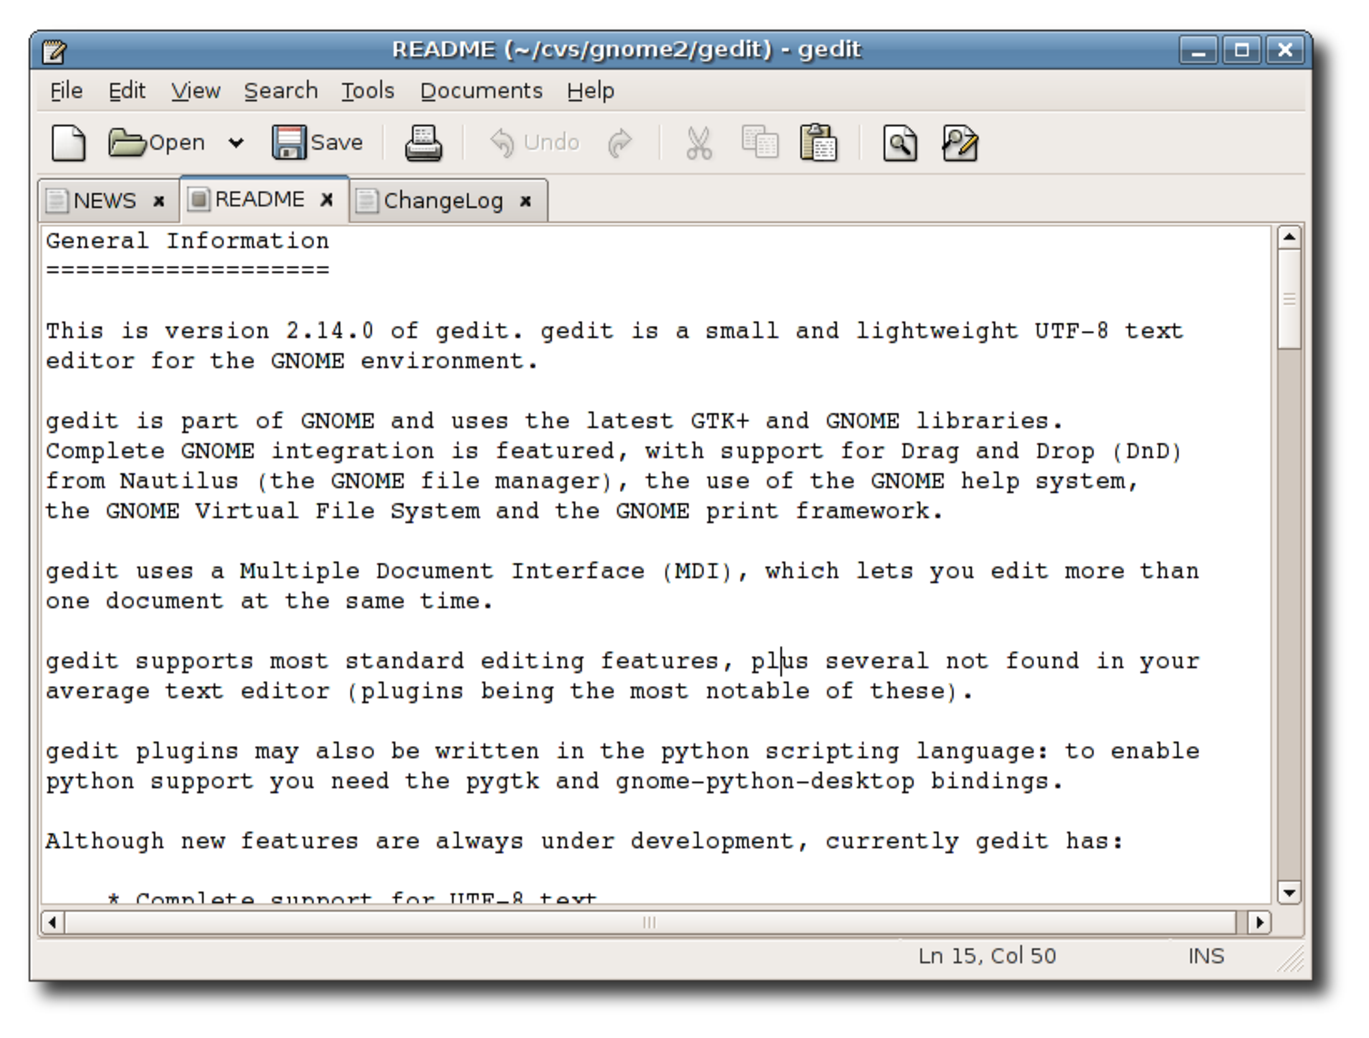
\includegraphics[scale=0.5]{gedit1.eps}<1> 
	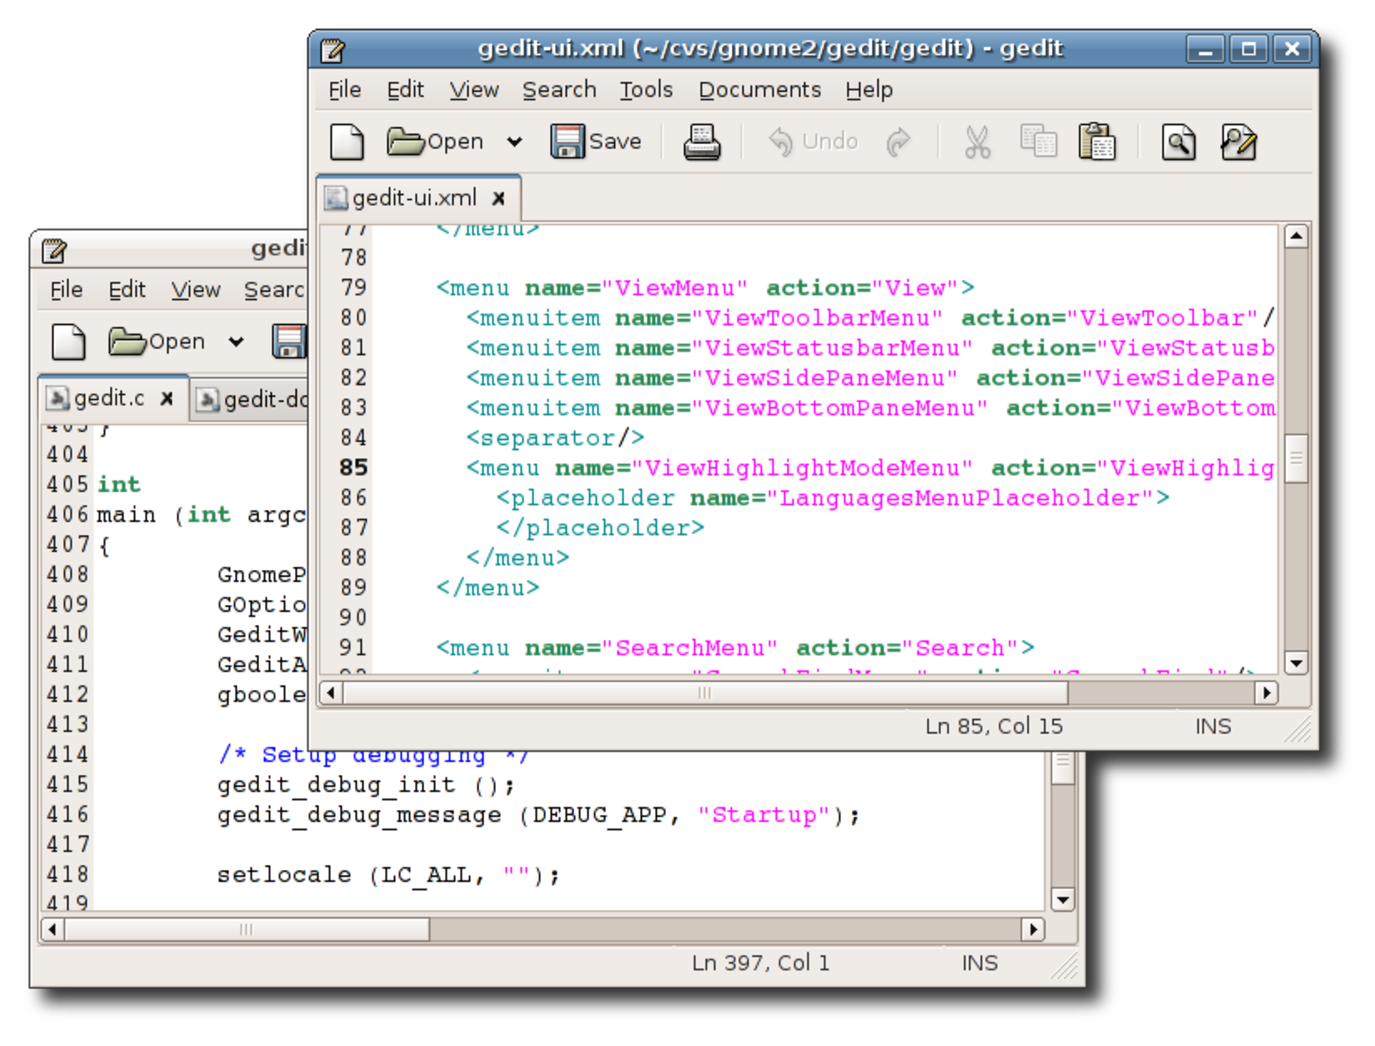
\includegraphics[scale=0.5]{gedit2.eps}<2>
	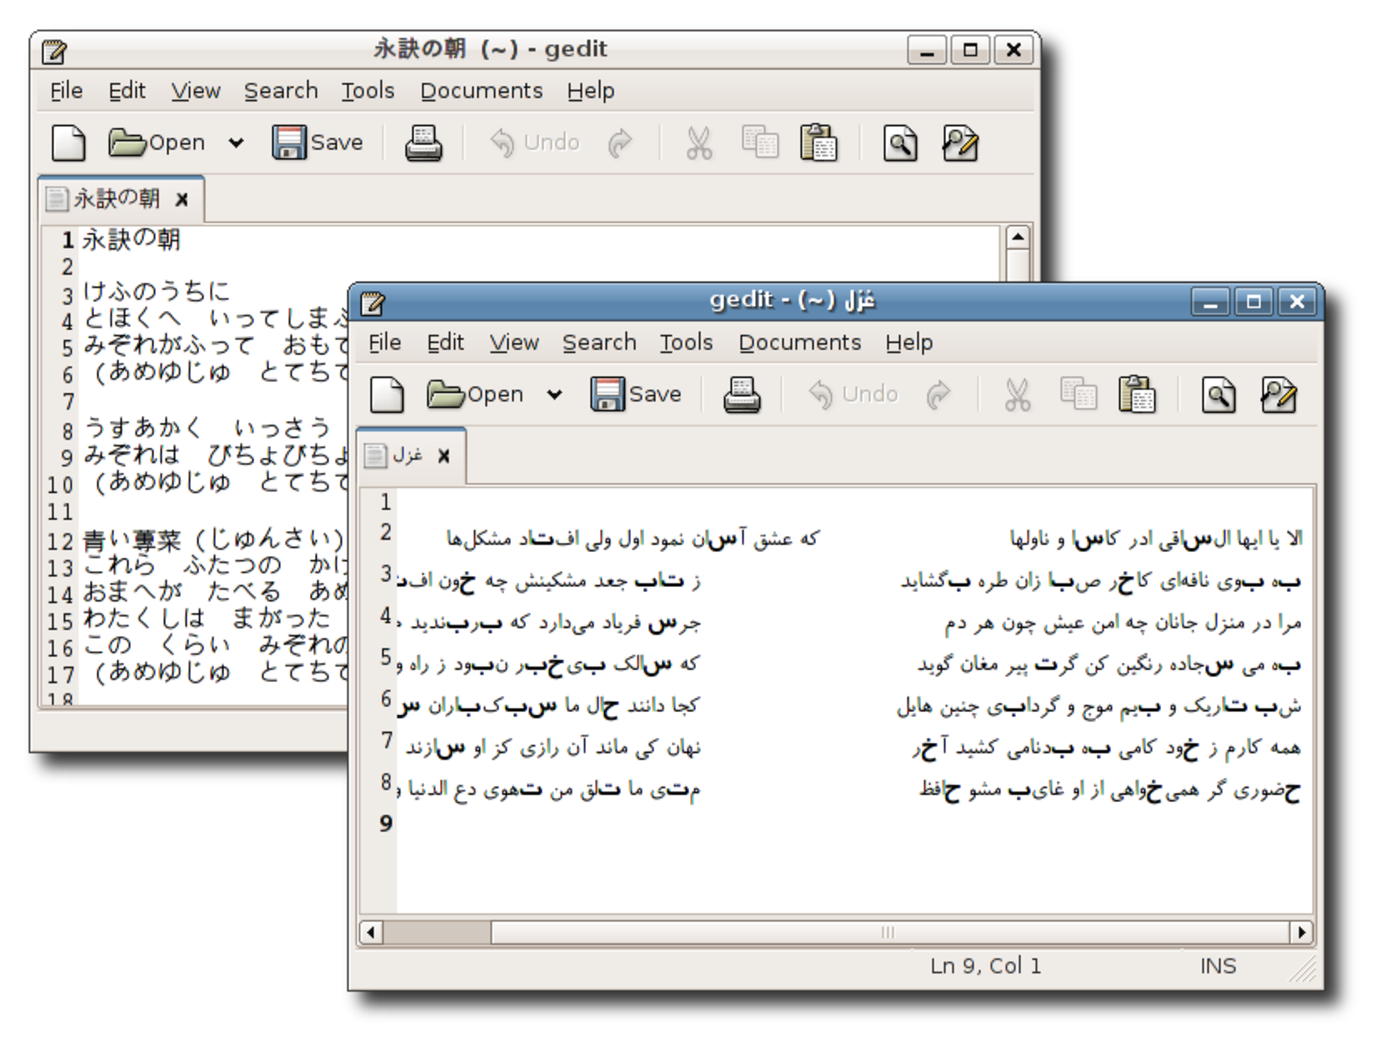
\includegraphics[scale=0.5]{gedit3.eps}<3>
	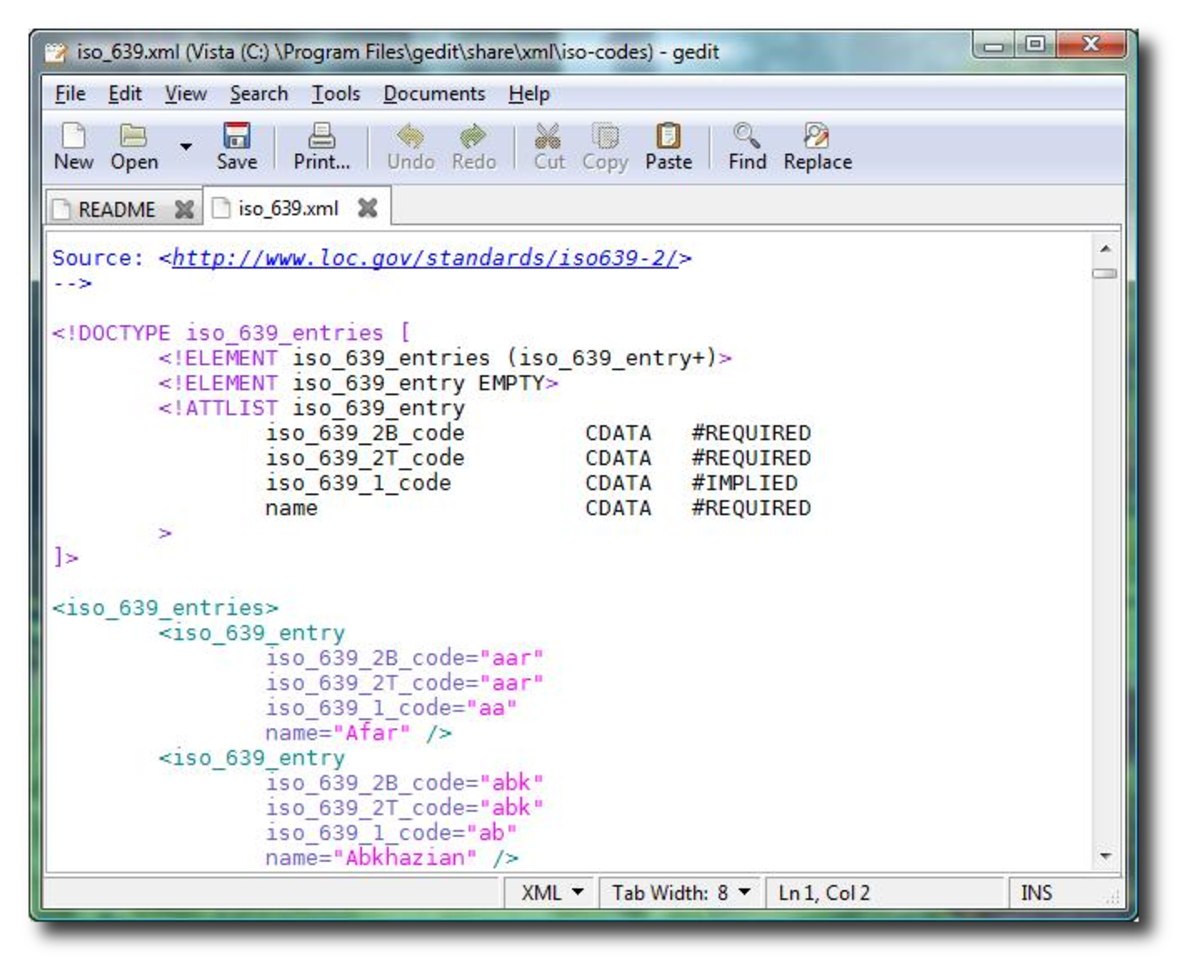
\includegraphics[scale=0.5]{gedit4.eps}<4>
	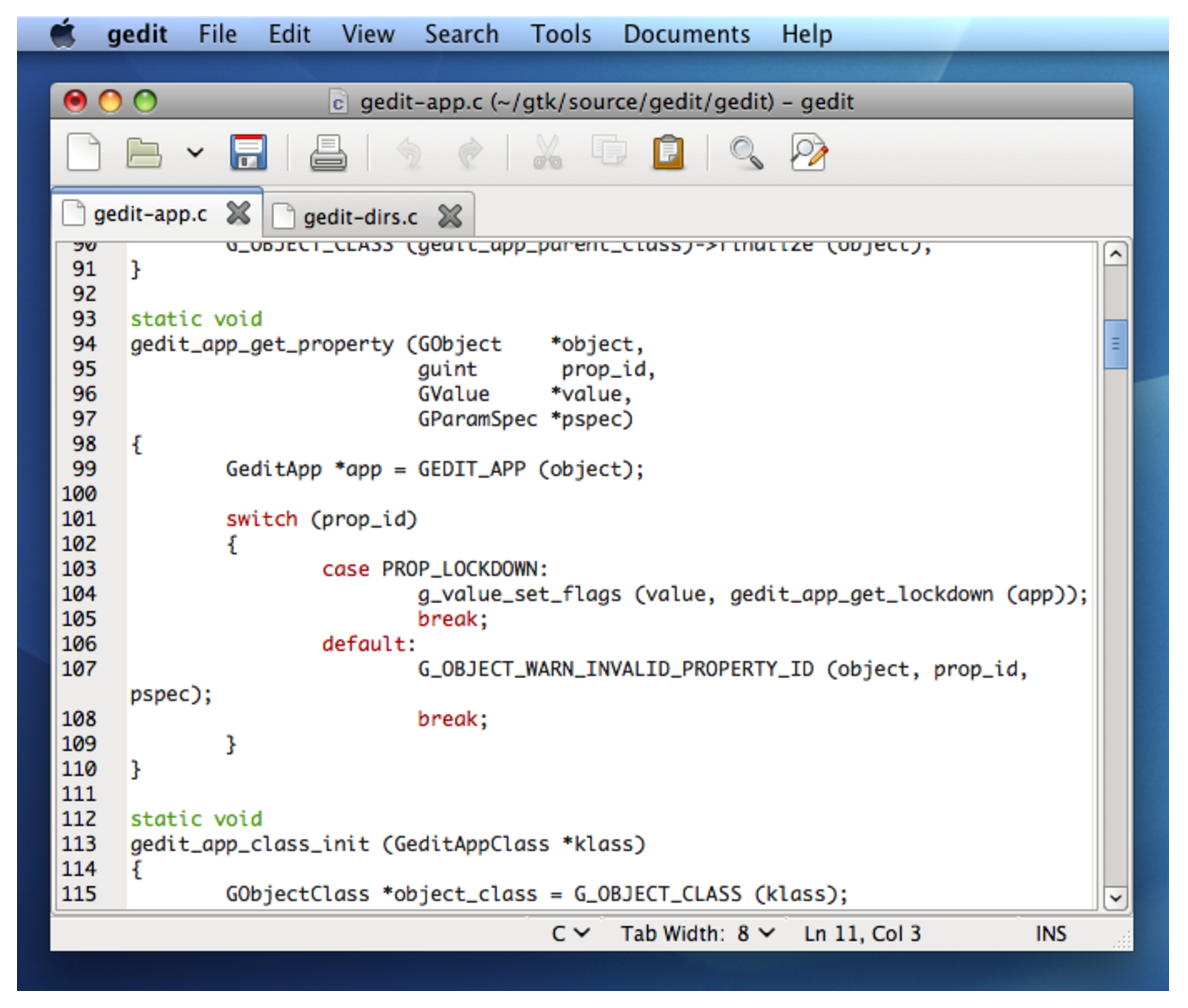
\includegraphics[scale=0.5]{gedit5.eps}<5>
\end{figure}
\end{frame}
\begin{frame}
\frametitle{El entorno Spyder2}
Spyder es un entorno de desarrollo integrado para el lenguaje Python con pruebas interactivas y funciones avanzadas de depuración, introspección y edición.
\\
\medskip
Spyder permite trabajar fácilmente con las mejores herramientas de la pila científica de Python en un entorno sencillo y potente.
\\
\medskip
\texttt{https://code.google.com/p/spyderlib/}
\end{frame}
\begin{frame}[fragile]
Estas son algunas de las características clave de Spyder:
\begin{enumerate}[<+->]
\item Cuadro de diálogo de administración de \texttt{PYTHONPATH} como de MATLAB (funciona con todas las consolas)
\item Editor de variables de entorno de usuario actual.
\item Enlaces directos a la documentación (Python, Matplotlib, NumPy, Spicy, etc.)
\item Enlace directo al lanzador de Python(x,y)
\item Enlaces directos a QtDesigner, QtLinguist y QtAssistant (documentación de Qt)
\end{enumerate}
\end{frame}
\begin{frame}
\begin{figure}
	\centering
	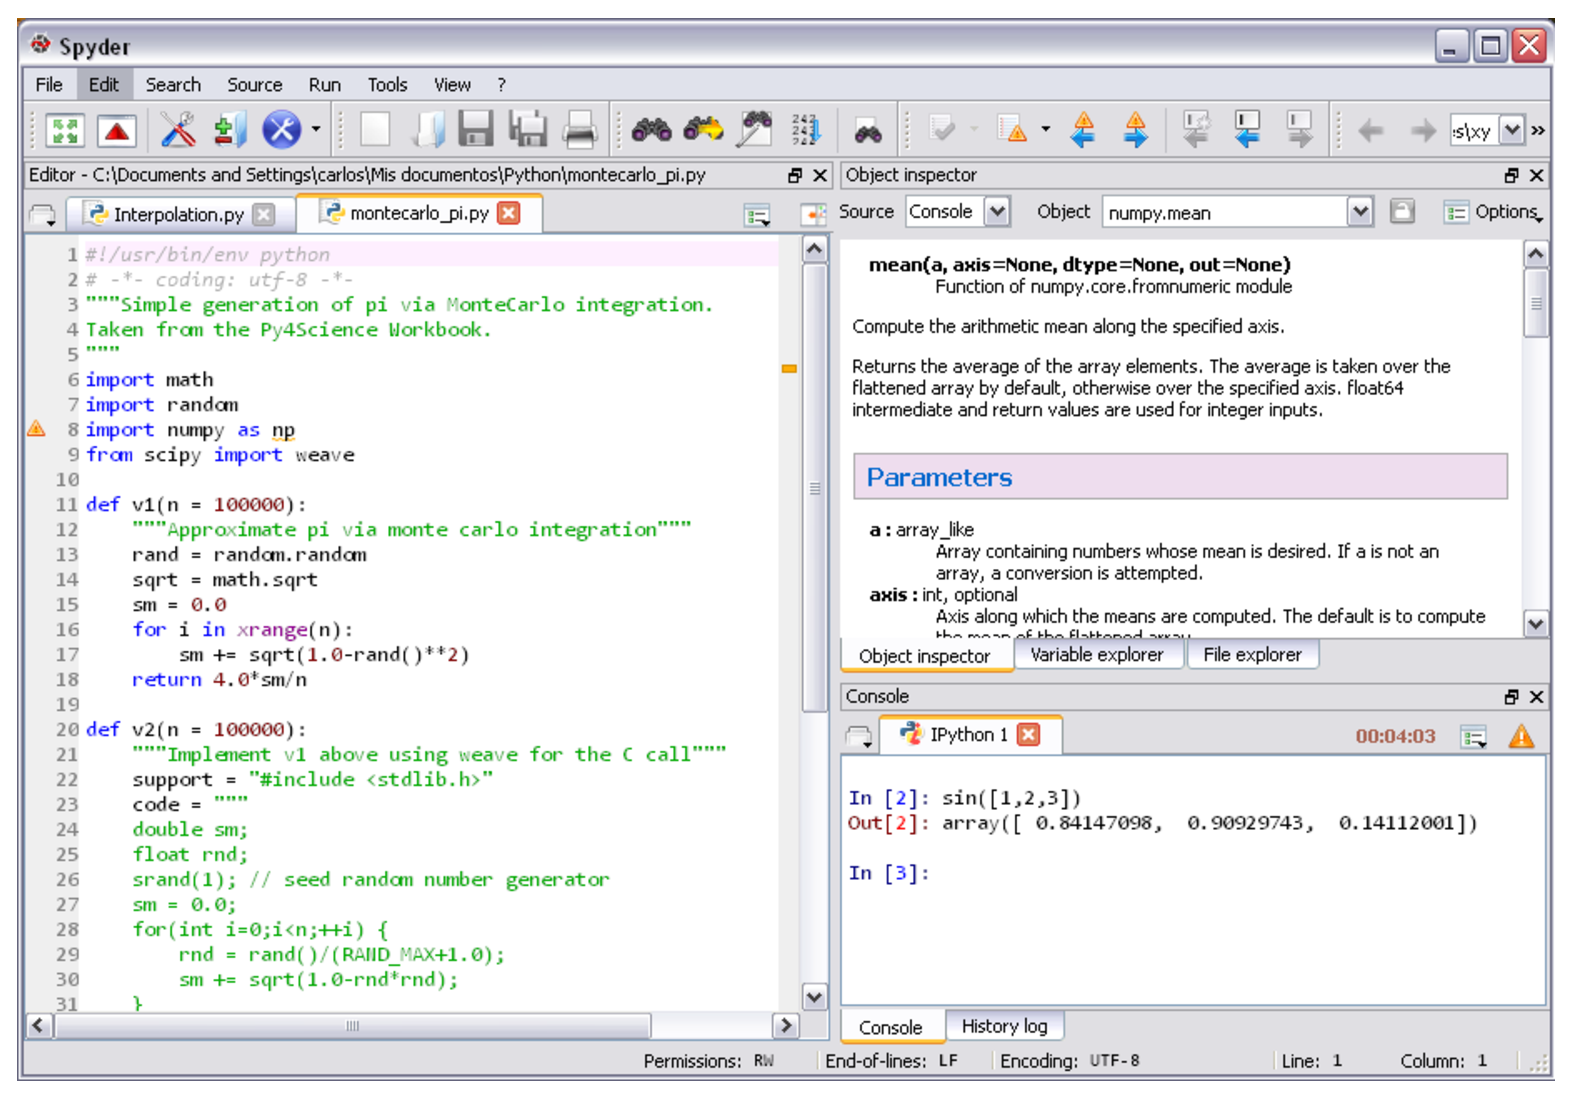
\includegraphics[scale=0.5]{spyder-windows.eps}<1>
	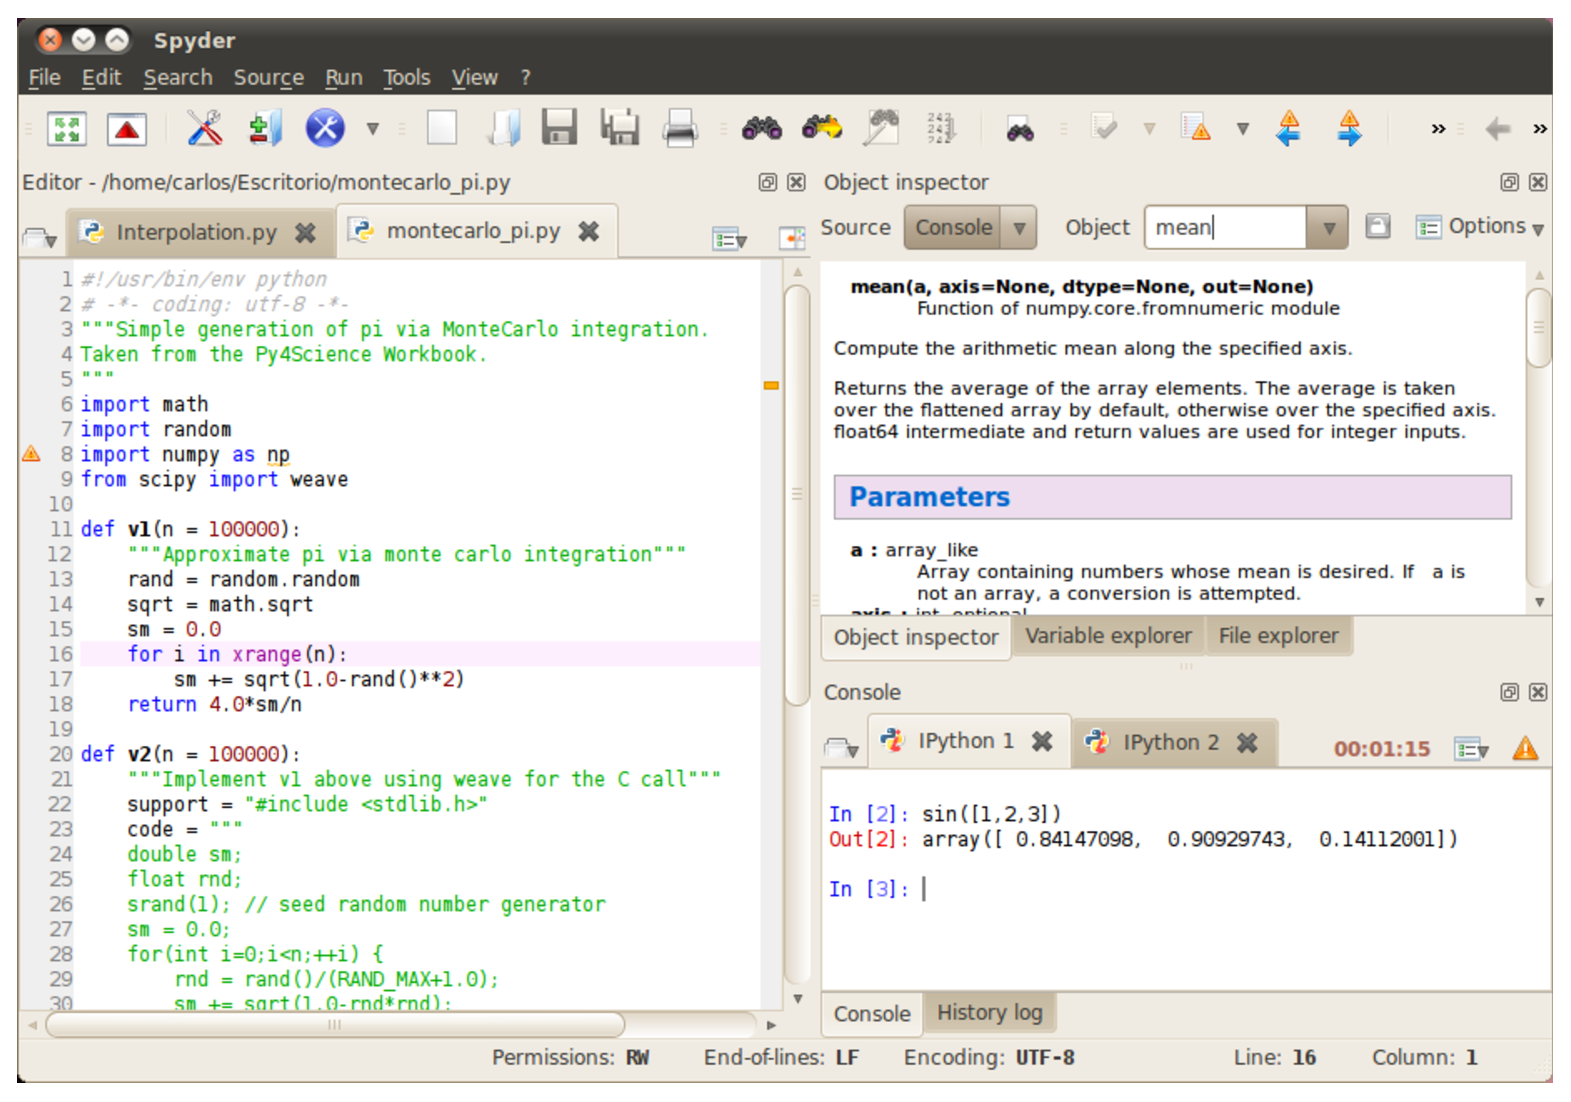
\includegraphics[scale=0.5]{spyder-linux.eps}<2> 
\end{figure}
\end{frame}
\begin{frame}
\frametitle{Otros IDEs para Python}
Pueden probar los IDE mencionados, pero también es importante señalar que hay otros entornos, cada uno con ciertas características que lo hacen particular. El punto es que si trabajan con uno, lo puedan explotar al máximo.
\\
\medskip
Una lista de otros IDEs para programar con Python, la pueden consultar en:
\\
\medskip
\texttt{https://wiki.python.org/moin/PythonEditors}
\end{frame}
\section{Graficación con Python}
\begin{frame}
\frametitle{Graficación con Python}
Una buena parte del trabajo que tendremos que hacer como físicos es utilizar un conjunto de datos que por si solos, no van a darnos información sobre un modelo o un fenómeno, por ello, será necesario usar gráficas.
\\
\medskip
Python incluye un módulo de graficación bastante versátil para generar gráficas y exportarlas a diferentes tipos de archivos.
\\
\medskip
La librería se llama \texttt{matplotlib}. Haremos algunos ejercicios para demostrar su potencia.
\end{frame}
\begin{frame}
\texttt{matplotlib.pyplot} es una colección de funciones de estilo de mando, de tal manera que matplotlib funciona a la manera de MATLAB. Cada instrucción \texttt{pyplot} aplica un cambio a una figura: por ejemplo, crear una figura, crear un área de trazado en una figura, trazar algunas líneas en un área de trazado, decorar con etiquetas, etc.
\end{frame}
\begin{frame}[fragile]
\frametitle{Ejecicio 1}
\begin{lstlisting}
import matplotlib.pyplot as plt
plt.plot([1,2,3,4])
plt.ylabel('algunos numeros')
plt.show()
\end{lstlisting}
\begin{figure}
	\centering
	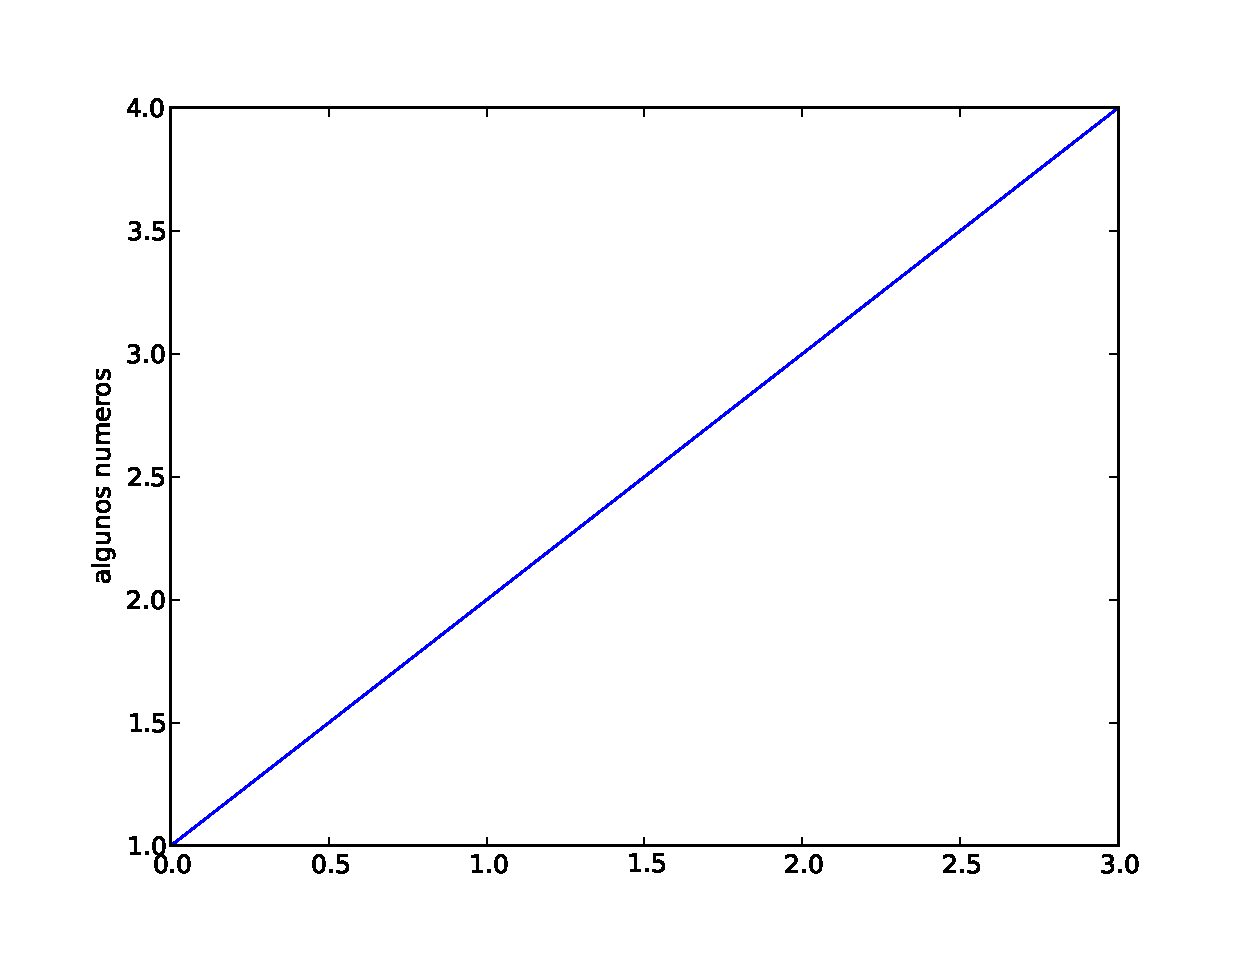
\includegraphics[scale=0.35]{plotEjercicio1.eps}<2> 
\end{figure}
\end{frame}
\begin{frame}
Te estarás preguntando por qué tenemos en el eje $x$ el rango $0-3$ y en el eje $y$ el rango  $1-4$.
\\
\medskip
Si proporcionamos una única lista o matriz en el comando \texttt{plot}, \texttt{matplotlib} asume que es una secuencia de valores de $y$, por lo que genera automáticamente los valores de $x$ para nosotros. Como los índices en Python comienzan en $0$, el vector $x$ por defecto tiene la misma longitud que $y$, pero inicia con 0. De ahí que los datos $x$ son $[0,1,2,3]$.
\end{frame}
\begin{frame}[fragile]
\frametitle{Ejecicio 2}
\begin{lstlisting}
import matplotlib.pyplot as plt
plt.plot([1,2,3,4], [1,4,9,16], 'ro')
plt.axis([0, 6, 0, 20])
plt.show()
\end{lstlisting}
\begin{figure}
	\centering
	\includegraphics[scale=0.35]{plotEjercicio2.eps}<2> 
\end{figure}
\end{frame}
\begin{frame}[fragile]
Por cada par $x$, $y$ de argumentos, existe un tercer argumento opcional, que es la cadena de formato que indica el color y tipo de línea.
\\
\medskip
Las letras y los símbolos de la cadena de formato son como en MATLAB, y concatenar una cadena de color con una cadena estilo de línea.
\\
\medskip
La cadena de formato por defecto es \verb|'b-'|, que es una línea de color azul.
\end{frame}
\begin{frame}[fragile]
\begin{tabular}{l | l}
carácter & descripción \\ \hline
\verb|'-'|	& línea sólida \\ \hline
\verb|'--'| & línea cortada \\ \hline
\verb|'-.'| & línea-punto \\ \hline
\verb|':'|	& línea de puntos \\ \hline
\verb|'.'|	& marca de punto \\ \hline
\verb|','|	& marca de pixel \\ \hline
\verb|'o'|	& marca de círculo \\ \hline
\verb|'v'|	& marca de triándulo hacia abajo \\ \hline
\verb|'^'|	& marca de triángulo hacia arriba
\end{tabular}
\end{frame}
\begin{frame}[fragile]
\begin{tabular}{l | l}
carácter & color \\ \hline
\verb|'b'| & azul \\ \hline
\verb|'g'| & verde \\ \hline
\verb|'r'| & rojo \\ \hline
\verb|'c'| & cyan \\ \hline
\verb|'m'| & magenta \\ \hline
\verb|'y'| & amarillo \\ \hline
\verb|'k'| & negro \\ \hline
\verb|'w'| & blanco
\end{tabular}
\end{frame}
\begin{frame}
\texttt{matplotlib} se limita a trabajar con listas, por lo que sería bastante acotado para el procesamiento y análisis numérico.
\\
\medskip
Por lo general, se utilizan los arreglos del módulo \texttt{numpy}. De hecho, todas las secuencias se convierten en matrices de \texttt{numpy} internamente.
\\
\medskip
El siguiente ejemplo ilustra un trazado de líneas con varios estilos diferentes en una sola instucción utilizando arreglos.
\end{frame}
\begin{frame}[fragile]
\frametitle{Ejecicio 3}
\begin{lstlisting}
import numpy as np
import matplotlib.pyplot as plt

t = np.arange(0., 5., 0.2)
plt.plot(t, t, 'r--', t, t**2, 'bs', t, t**3, 'g^')
plt.show()
\end{lstlisting}
\end{frame}
\begin{frame}[fragile]
\begin{figure}
	\centering
	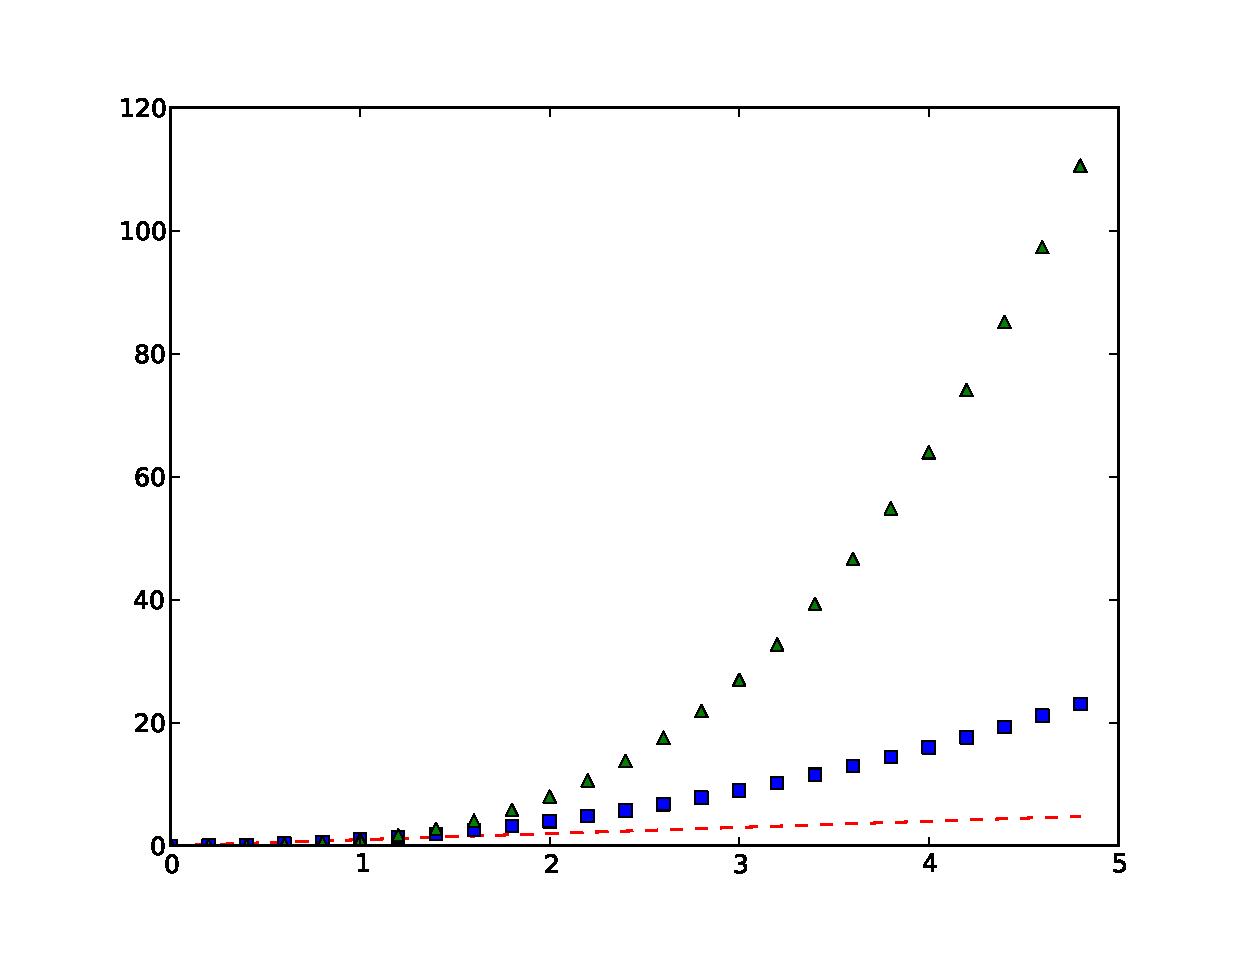
\includegraphics[scale=0.5]{plotEjercicio3.eps}
\end{figure}
\end{frame}
\begin{frame}[fragile]
\frametitle{Ejercicio 4}
Trabajando con múltiples gráficas
\begin{lstlisting}
import numpy as np
import matplotlib.pyplot as plt

def f(t):
    return np.exp(-t) * np.cos(2*np.pi*t)

t1 = np.arange(0.0, 5.0, 0.1)
t2 = np.arange(0.0, 5.0, 0.02)

plt.figure(1)
plt.subplot(211)
plt.plot(t1, f(t1), 'bo', t2, f(t2), 'k')

plt.subplot(212)
plt.plot(t2, np.cos(2*np.pi*t2), 'r--')
\end{lstlisting}
\end{frame}
\begin{frame}[fragile]
\begin{figure}
	\centering
	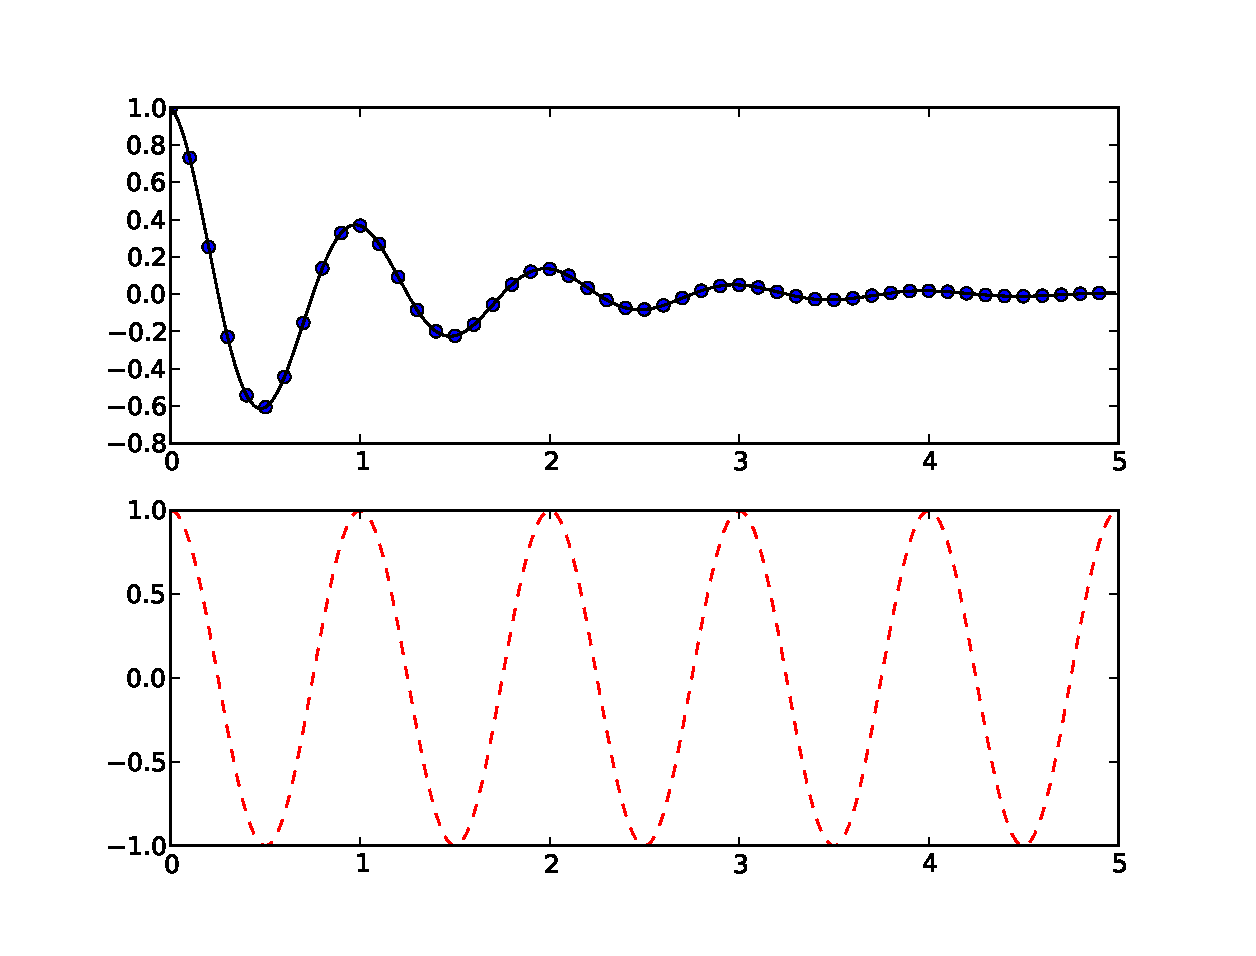
\includegraphics[scale=0.5]{plotEjercicio4.eps}
\end{figure}
\end{frame}
\begin{frame}
El comando \texttt{figure()} aquí es opcional, ya \texttt{figure(1)} se crea de forma predeterminada, así mismo \texttt{subplot(111)} se crea de forma predeterminada si no se especifica manualmente un eje.
\\
\medskip
El comando \texttt{subplot()} especifica \texttt{numrows, numcols, fignum} donde \texttt{fignum} varía en rango de 1 a \texttt{numrows * numcols}. Las comas en el comando \texttt{subplot()} son opcionales si \texttt{numrows * numcols} $<10$. Por tanto \texttt{subplot(211)} es idéntica a la \texttt{subplot(2,1,1)}.
\end{frame}
\begin{frame}[fragile]
\frametitle{Ejercicio 5}
\begin{lstlisting}
import matplotlib.pyplot as plt

plt.figure(1)                
plt.subplot(211)         
plt.plot([1,2,3])
plt.subplot(212)         
plt.plot([4,5,6])


plt.figure(2)                
plt.plot([4,5,6])           

plt.figure(1)                
plt.subplot(211)         
plt.title('Tan facil como 1,2,3')
plt.show()
\end{lstlisting}
\end{frame}
\begin{frame}[fragile]
\begin{figure}
	\centering
	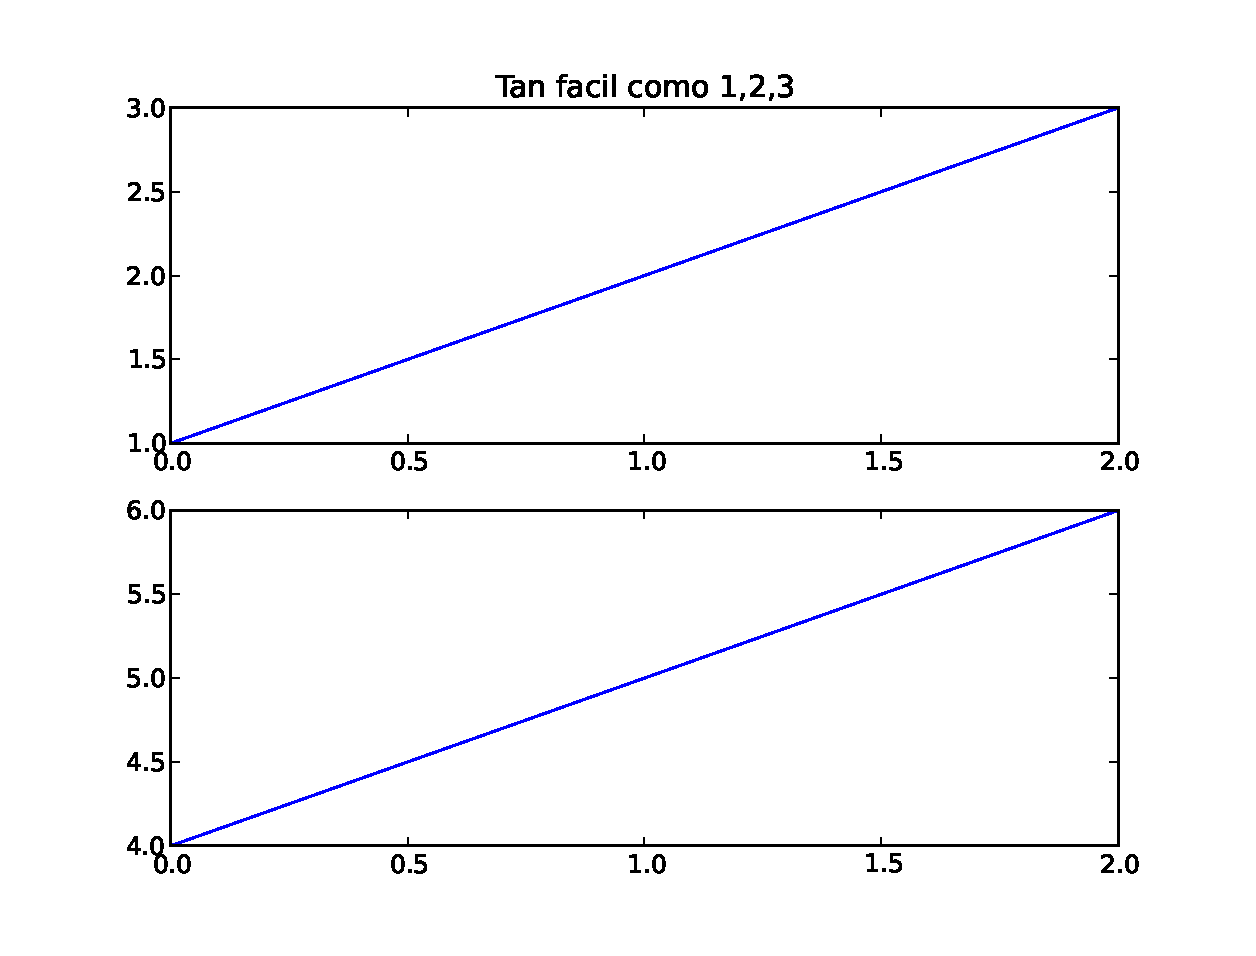
\includegraphics[scale=0.5]{plotEjercicio5_1.eps}<1>
	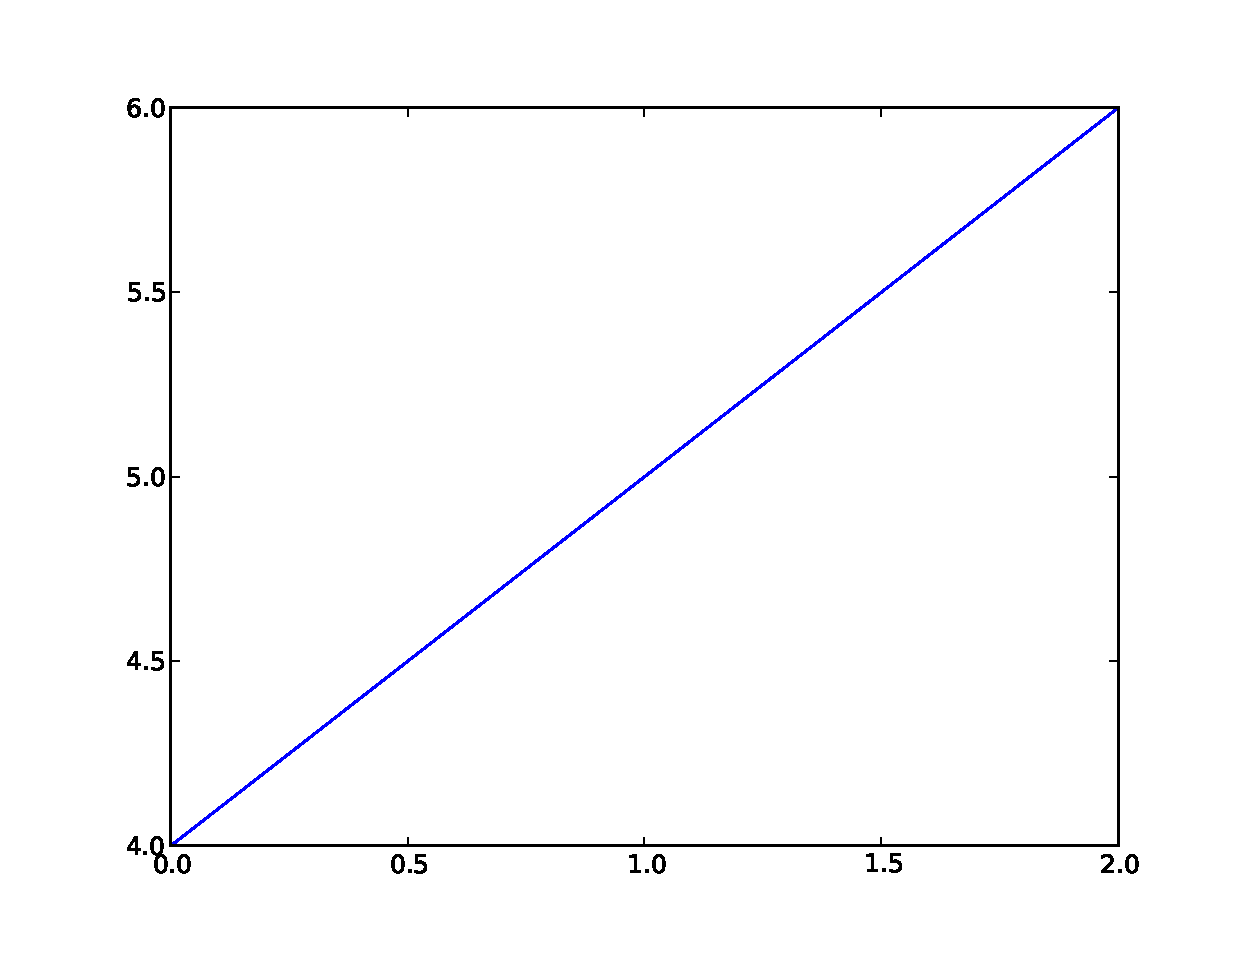
\includegraphics[scale=0.5]{plotEjercicio5_2.eps}<2>
\end{figure}
\end{frame}
\section{Arreglos}
\begin{frame}
\frametitle{Lo que podemos hacer con los arreglos}
\begin{enumerate}
\item Crear arreglos.
\item Operaciones con arreglos.
\item Funciones sobre arreglos.
\item Obtener elementos de un arreglo.
\item Algunos métodos convenientes.
\item Productos con arreglos.
\begin{enumerate}
\item Producto interno (vector-vector)
\item Producto matriz-vector.
\item Producto matriz-matriz.
\end{enumerate}
\end{enumerate}
\end{frame}
\begin{frame}
\frametitle{Repaso express sobre arreglos}
Las estructuras de datos que hemos visto hasta ahora permiten manipular datos de manera muy flexible. Combinándolas y anidándolas, es posible organizar información de manera estructurada para representar sistemas del mundo real.
\end{frame}
\begin{frame}
En muchas aplicaciones en Ciencias, más importante que la organización de los datos es la capacidad de hacer muchas operaciones a la vez sobre grandes conjuntos de datos numéricos de manera eficiente. Algunos ejemplos de problemas que requieren manipular grandes secuencias de números son: la predicción del clima, simulación, graficación de modelos, la construcción de edificios, y el análisis de indicadores financieros entre muchos otros.
\end{frame}
\begin{frame}
La estructura de datos que sirve para almacenar estas grandes secuencias de números (generalmente de tipo float) es el \textbf{arreglo}.
\\
\bigskip
Los arreglos tienen algunas similitudes con las listas:
\begin{itemize}
\item los elementos tienen un orden y se pueden acceder mediante su posición.
\item los elementos se pueden recorrer usando un ciclo \texttt{for}.
\end{itemize}
\end{frame}
\begin{frame}
Sin embargo, también tienen algunas restricciones:
\begin{itemize}
\item todos los elementos del arreglo deben tener el mismo tipo.
\item en general, el tamaño del arreglo es fijo (no van creciendo dinámicamente como las listas).
\item se ocupan principalmente para almacenar datos numéricos.
\end{itemize}
\end{frame}
\begin{frame}
Los arreglos son los equivalentes en programación de las matrices y vectores en matemáticas. Precisamente, una gran motivación para usar arreglos es que hay mucha teoría detrás de ellos que puede ser usada en el diseño de algoritmos para resolver problemas verdaderamente interesantes.
\end{frame}
\begin{frame}[fragile]
\frametitle{Crear arreglos}
El módulo que provee las estructuras de datos y las funciones para trabajar con arreglos es \texttt{NumPy}.
\begin{verbatim}
from numpy import array
\end{verbatim}
Como estaremos usando frecuentemente muchas funciones de este módulo, conviene importarlas todas de una vez usando la siguiente sentencia:
\begin{verbatim}
from numpy import *
\end{verbatim}
\end{frame}
\begin{frame}[fragile]
El tipo de datos de los arreglos se llama \textcolor{blue}{array}. Para crear un arreglo nuevo, se puede usar la función array pasándole como parámetro la lista de valores que deseamos agregar al arreglo:
\begin{exampleblock}{}<2->
\pause
\verb|>>> a = array([6, 1, 3, 9, 8])| \\
\pause
\verb|>>> a|  \\
\pause
\verb|array([6, 1, 3, 9, 8])|
\end{exampleblock}
\pause
Todos los elementos del arreglo tienen exactamente el mismo tipo. Para crear un arreglo de números reales, basta con que uno de los valores lo sea:
\pause
\begin{exampleblock}{}<3->
\pause
\verb|>>> b = array([6.0, 1, 3, 9, 8])| \\
\pause
\verb|>>> b| \\
\pause
\verb|array([ 6.,  1.,  3.,  9.,  8.])| 
\end{exampleblock}
\end{frame}
\begin{frame}[fragile]
Otra opción es convertir el arreglo a otro tipo usando el método \texttt{astype:}
\begin{exampleblock}{}<2->
\verb|>>> a| \\
\pause
\verb|array([6, 1, 3, 9, 8])| \\
\pause
\verb|>>> a.astype(float)| \\
\pause
\verb|array([ 6.,  1.,  3.,  9.,  8.])| \\
\pause
\verb|>>> a.astype(complex)| \\
\pause
\verb|array([ 6.+0.j,  1.+0.j,  3.+0.j,  9.+0.j,  8.+0.j])|
\end{exampleblock}
\end{frame}
\begin{frame}[fragile]
Hay muchas formas de arreglos que aparecen a menudo en la práctica, por lo que existen funciones especiales para crearlos:
\begin{itemize}[<+->]
\item \texttt{zeros(n)} crea un arreglo de $n$ ceros.
\item \texttt{ones(n)} crea un arreglo de $n$ unos.
\item \texttt{arange(a, b, c)} crea un arreglo de forma similar a la función \texttt{range}, con las diferencias que $a$, $b$ y $c$ pueden ser reales, y que el resultado es un arreglo y no una lista.
\item \texttt{linspace(a, b, n)} crea un arreglo de $n$ valores equiespaciados entre $a$ y $b$.
\end{itemize}
\end{frame}
\begin{frame}[fragile]
\begin{exampleblock}{}<2->
\verb|>>> zeros(6)| \\
\pause
\verb|array([ 0.,  0.,  0.,  0.,  0.,  0.])| \\
\pause
\verb|>>> ones(5)| \\
\pause
\verb|array([ 1.,  1.,  1.,  1.,  1.])| \\
\pause
\verb|>>> arange(3.0, 9.0)| \\
\pause
\verb|array([ 3.,  4.,  5.,  6.,  7.,  8.])|\\
\pause
\verb|>>> linspace(1, 2, 5)| \\
\pause
\verb|array([ 1.  ,  1.25,  1.5 ,  1.75,  2.  ])|
\end{exampleblock}
\end{frame}
\begin{frame}[fragile]
\frametitle{Operaciones con arreglos}
Las limitaciones que tienen los arreglos respecto de las listas son compensadas por la cantidad de operaciones convenientes que permiten realizar sobre ellos.
\\
\bigskip
Las operaciones aritméticas entre arreglos se aplican elemento a elemento:
\fontsize{12}{12}\selectfont
\begin{exampleblock}{}
\verb|>>> a = array([55, 21, 19, 11,  9])|
\verb|>>> b = array([12, -9,  0, 22, -9])|
\end{exampleblock}
\begin{exampleblock}{sumar los dos arreglos elemento a elemento}<2->
\verb|>>> a + b| \\
\verb|array([67, 12, 19, 33,  0])|
\end{exampleblock}
\end{frame}
\begin{frame}[fragile]
\begin{exampleblock}{multiplicar por $0.1$ todos los elementos}
\verb|>>> 0.1 * a| \\
\verb|array([ 5.5,  2.1,  1.9,  1.1,  0.9])|
\end{exampleblock}
\begin{exampleblock}{restar $9.0$ a todos los elementos}<2->
\verb|>>> a - 9.0| \\
\verb|array([ 46.,  12.,  10.,   2.,   0.])|
\end{exampleblock}
Note que si quisiéramos hacer estas operaciones usando listas, necesitaríamos usar un ciclo para hacer las operaciones elemento a elemento.
\end{frame}
\begin{frame}[fragile]
Las operaciones relacionales también se aplican elemento a elemento, y devuelven un arreglo de valores booleanos:
\fontsize{12}{12}\selectfont
\begin{exampleblock}{}<2->
\verb|>>> a = array([5.1, 2.4, 3.8, 3.9])| \\
\verb|>>> b = array([4.2, 8.7, 3.9, 0.3])| \\
\verb|>>> c = array([5, 2, 4, 4]) + array([1, 4, -2, -1])/10.0|\\
\pause
\verb|>>> a < b| \\
\pause
\verb|array([False,  True,  True, False], dtype=bool)| \\
\pause
\verb|>>> a == c| \\
\pause
\verb|array([ True,  True,  True,  True], dtype=bool)|
\end{exampleblock}
\end{frame}
\begin{frame}[fragile]
Para reducir el arreglo de booleanos a un único valor, se puede usar las funciones \texttt{any} y \texttt{all.any} devuelve \texttt{True} si al menos uno de los elementos es verdadero, mientras que \texttt{all} devuelve \texttt{True} sólo si todos lo son (del inglés, \texttt{any} signfica \textit{alguno}, y \texttt{all} significa \textit{todos}):
\begin{exampleblock}{}<2->
\verb|>>> any(a < b)| \\
\pause
\verb|True| \\
\pause
\verb|>>> any(a == b)| \\
\pause
\verb|False| \\
\pause
\verb|>>> all(a == c)| \\
\pause
\verb|True|
\end{exampleblock}
\end{frame}
\begin{frame}[fragile]
\frametitle{Funciones sobre arreglos}
\texttt{NumPy} provee muchas funciones matemáticas que también operan elemento a elemento.
\begin{exampleblock}{}<2->
\verb|>>> from numpy import linspace, pi, sin| \\
\verb|>>> x = linspace(0, pi/2, 9)| \\
\fontsize{10}{10}\selectfont
\verb|>>> x| \\
\pause
\verb|array([ 0.        ,  0.19634954,  0.39269908,|\\ 
\verb|        0.58904862,  0.78539816,  0.9817477 ,|\\
\verb|        1.17809725,  1.37444679,  1.57079633])| \\
\verb|>>> sin(x)| \\
\pause
\verb|array([ 0.        ,  0.19509032,  0.38268343,| \\
\verb|        0.55557023,  0.70710678,  0.83146961,| \\
\verb|        0.92387953,  0.98078528,  1.        ])|
\end{exampleblock}
Como puede ver, los valores obtenidos van de 0 a 1, que es justamente como se comporta la función seno en el intervalo $[0, \pi/2]$.
\end{frame}
\begin{frame}[fragile]
Aquí también se hace evidente otra de las ventajas de los arreglos: al mostrarlos en la consola o al imprimirlos, los valores aparecen perfectamente alineados. Con las listas, esto no ocurre:
\fontsize{12}{12}\selectfont
\begin{exampleblock}{}
\verb|>>> list(sin(x))| \\
\pause
\verb|[0.0, 0.19509032201612825, 0.38268343236508978, 0.5555702330| \\
\verb|1960218, 0.70710678118654746, 0.83146961230254524, 0.9238795| \\
\verb|3251128674, 0.98078528040323043, 1.0]|
\end{exampleblock}
\end{frame}
\begin{frame}[fragile]
\frametitle{Arreglos aleatorios}
\texttt{NumPy} contiene a su vez otros módulos que proveen funcionalidad adicional a los arreglos y funciones básicos.
\\
\bigskip
El módulo \texttt{numpy.random} provee funciones para crear números aleatorios (es decir, generados al azar), de las cuales la más usada es la función \texttt{random}, que entrega un arreglo de números al azar distribuidos uniformemente entre 0 y 1:
\\
\bigskip
\verb|>>> from numpy.random import random|
\end{frame}
\begin{frame}[fragile]
\fontsize{12}{12}\selectfont
\begin{exampleblock}{}
\verb|>>> random(3)| \\
\pause
\verb|array([ 0.53077263,  0.22039319,  0.81268786])| \\
\verb|>>> random(3)| \\
\pause
\verb|array([ 0.07405763,  0.04083838,  0.72962968])| \\
\pause
\verb|>>> random(3)| \\
\pause
\verb|array([ 0.51886706,  0.46220545,  0.95818726])|
\end{exampleblock}
\end{frame}
\begin{frame}[fragile]
\frametitle{Obtener elementos de un arreglo}
Cada elemento del arreglo tiene un índice, al igual que en las listas. El primer elemento tiene índice $0$. Los elementos también pueden numerarse desde el final hasta el principio usando índices negativos. El último elemento tiene índice $-1$:
\fontsize{12}{12}\selectfont
\begin{exampleblock}{}<2->
\verb|>>> a = array([6.2, -2.3, 3.4, 4.7, 9.8])| \\
\pause
\verb|>>> a[0]| \\
\pause
\verb|6.2| \\
\pause
\verb|>>> a[1]| \\
\pause
\verb|-2.3| \\
\pause
\verb|>>> a[-2]| \\
\pause
\verb|4.7| \\
\pause
\verb|>>> a[3]| \\
\pause
\verb|4.7|
\end{exampleblock}
\end{frame}
\begin{frame}[fragile]
Una sección del arreglo puede ser obtenida usando el operador de rebanado $a[i:j]$. Los índices $i$ y $j$ indican el rango de valores que serán devueltos:
\begin{exampleblock}{}<2->
\verb|>>> a| \\
\pause
\verb|array([ 6.2, -2.3,  3.4,  4.7,  9.8])| \\
\pause
\verb|>>> a[1:4]| \\
\pause
\verb|array([-2.3,  3.4,  4.7])| \\
\pause
\verb|>>> a[2:-2]| \\
\pause
\verb|array([ 3.4])|
\end{exampleblock}
\end{frame}
\begin{frame}[fragile]
Si el primer índice es omitido, el rebanado comienza desde el principio del arreglo. Si el segundo índice es omitido, el rebanado termina al final del arreglo:
\begin{exampleblock}{}<2->
\verb|>>> a[:2]| \\
\pause
\verb|array([ 6.2, -2.3])| \\
\pause
\verb|>>> a[2:]| \\
\pause
\verb|array([ 3.4,  4.7,  9.8])|
\end{exampleblock}
\end{frame}
\begin{frame}[fragile]
Un tercer índice puede indicar cada cuántos elementos serán incluidos en el resultado:
\fontsize{12}{12}\selectfont
\begin{exampleblock}{}<2->
\verb|>>> a = linspace(0, 1, 9)| \\
\pause
\verb|>>> a| \\
\pause
\verb|array([ 0.   ,  0.125,  0.25 ,  0.375,  0.5  ,  0.625,  0.75 ,  0.875,  1.   ])| \\
\pause
\verb|>>> a[1:7:2]| \\
\pause
\verb|array([ 0.125,  0.375,  0.625])| \\
\pause
\verb|>>> a[::3]| \\
\pause
\verb|array([ 0.   ,  0.375,  0.75 ])| \\
\pause
\verb|>>> a[-2::-2]| \\
\pause
\verb|array([ 0.875,  0.625,  0.375,  0.125])| \\
\pause
\verb|>>> a[::-1]| \\
\pause
\verb|array([ 1.   ,  0.875,  0.75 ,  0.625,  0.5  ,  0.375,  0.25 ,  0.125,  0.   ])|
\end{exampleblock}
\end{frame}
\begin{frame}[fragile]
Una manera simple de recordar cómo funciona el rebanado es considerar que los índices no se refieren a los elementos, sino a los espacios entre los elementos:
\fontsize{12}{12}\selectfont
\begin{exampleblock}{}<2->
\verb|>>> b = array([17.41, 2.19, 10.99, -2.29, 3.86, 11.10])| \\
\pause
\verb|>>> b[2:5]| \\
\pause
\verb|array([ 10.99,  -2.29,   3.86])| \\
\pause
\verb|>>> b[:5]| \\
\pause
\verb|array([ 17.41,   2.19,  10.99,  -2.29,   3.86])| \\
\pause
\verb|>>> b[1:1]| \\
\pause
\verb|array([], dtype=float64)| \\
\pause
\verb|>>> b[1:5:2]| \\
\pause
\verb|array([ 2.19, -2.29])|
\end{exampleblock}
\end{frame}
\begin{frame}[fragile]
\frametitle{Algunos métodos convenientes}
Los arreglos proveen algunos métodos útiles que conviene conocer.
\\
\bigskip
Los métodos \texttt{min} y \texttt{max}, entregan respectivamente el mínimo y el máximo de los elementos del arreglo:
\begin{exampleblock}{}<2->
\verb|>>> a = array([4.1, 2.7, 8.4, pi, -2.5, 3, 5.2])| \\
\pause
\verb|>>> a.min()| \\
\pause
\verb|-2.5| \\
\pause
\verb|>>> a.max()| \\
\pause
\verb|8.4000000000000004|
\end{exampleblock}
\end{frame}
\begin{frame}[fragile]
Los métodos \texttt{argmin} y \texttt{argmax} entregan respectivamente la posición del mínimo y del máximo:
\begin{exampleblock}{}<2->
\verb|>>> a.argmin()| \\
\pause
\verb|4| \\
\pause
\verb|>>> a.argmax()| \\
\pause
\verb|2|
\end{exampleblock}
\end{frame}
\begin{frame}[fragile]
Los métodos \texttt{sum} y \texttt{prod} entregan respectivamente la suma y el producto de los elementos:
\begin{exampleblock}{}<2->
\verb|>>> a.sum()| \\
\pause
\verb|24.041592653589795| \\
\pause
\verb|>>> a.prod()| \\
\pause
\verb|-11393.086289208301|
\end{exampleblock}
\end{frame}
\begin{frame}
\frametitle{Productos entre arreglos}
Recordemos que vector es sinónimo de arreglo de una dimensión, y matriz es sinónimo de arreglo de dos dimensiones.
\end{frame}
\begin{frame}[fragile]
\frametitle{Producto interno (vector-vector)}
El producto interno entre dos vectores se obtiene usando la función \texttt{dot} provista por NumPy:
\fontsize{12}{12}\selectfont
\begin{exampleblock}{}
\verb|>>> a = array([-2.8 , -0.88,  2.76,  1.3 ,  4.43])| \\
\verb|>>> b = array([ 0.25, -1.58,  1.32, -0.34, -4.22])| \\
\pause
\verb|>>> dot(a, b)| \\
\pause
\verb|-14.803|
\end{exampleblock}
\end{frame}
\begin{frame}[fragile]
El producto interno es una operación muy común. Por ejemplo, suele usarse para calcular totales:
\fontsize{12}{12}\selectfont
\begin{exampleblock}{}
\verb|>>> precios = array([200, 100, 500, 400, 400, 150])|
\verb|>>> cantidades = array([1, 0, 0, 2, 1, 0])|
\pause
\verb|>>> total_a_pagar = dot(precios, cantidades)|
\pause
\verb|>>> total_a_pagar|
\pause
\verb|1400|
\end{exampleblock}
También se usa para calcular promedios ponderados:
\begin{exampleblock}{}
\verb|>>> notas = array([45, 98, 32])| \\
\pause
\verb|>>> ponderaciones = array([30, 30, 40]) / 100.| \\
\pause
\verb|>>> nota_final = dot(notas, ponderaciones)| \\
\pause
\verb|>>> nota_final| \\
\verb|55.7|
\end{exampleblock}
\end{frame}
\begin{frame}[fragile]
\frametitle{Producto matriz-vector}
El producto matriz-vector es el vector de los productos internos. El producto matriz-vector puede ser visto simplemente como varios productos internos calculados de una sola vez.
\\
\bigskip
Esta operación también es obtenida usando la función \texttt{dot} entre las filas de la matriz y el vector:
\fontsize{12}{12}\selectfont
\begin{exampleblock}{}
\verb|>>> a = array([[-0.6,  4.8, -1.2],| \\
\verb|               [-2. , -3.6, -2.1],| \\
\verb|               [ 1.7,  4.9,  0. ]])| \\
\verb|>>> x = array([-0.6, -2. ,  1.7])| \\
\pause
\verb|>>> dot(a, x)| \\
\pause
\verb|array([-11.28,   4.83, -10.82])|
\end{exampleblock}
\end{frame}
\begin{frame}[fragile]
\frametitle{Producto matriz-matriz}
\fontsize{12}{12}\selectfont
El producto matriz-matriz es la matriz de los productos internos entre las filas de la primera matriz y las columnas de la segunda.
\begin{exampleblock}{}
\verb|>>> a = array([[ 2,  8],| \\
\verb|               [-3,  7],| \\
\verb|               [-8, -5]])| \\
\verb|>>> b array([[-3, -5, -6, -3],| \\
\verb|             [-9, -2,  3, -3]])| \\
\pause
\verb|>>> dot(a, b)| \\
\pause
\verb|array([[-78, -26,  12, -30],|\\
\verb|       [-54,   1,  39, -12],| \\
\verb|       [ 69,  50,  33,  39]])| \\
\end{exampleblock}
\end{frame}
\begin{frame}
La multiplicación de matrices puede ser vista como varios productos matriz-vector (usando como vectores todas las filas de la segunda matriz), calculados de una sola vez.
\end{frame}
\begin{frame}
En resumen, al usar la función \texttt{dot}, la estructura del resultado depende de cuáles son los parámetros pasados:
\begin{enumerate}[<+->]
\item \texttt{dot}(vector, vector) $\rightarrow$ número.
\item \texttt{dot}(matriz, vector) $\rightarrow$ vector.
\item \texttt{dot}(matriz, matriz) $\rightarrow$ matriz.
\end{enumerate}
\end{frame}
\section{Solución de sistemas de ecuaciones}
\begin{frame}
\frametitle{Solución de sistemas lineales}
\fontsize{12}{12}\selectfont
Un problema recurrente en Ciencias consiste en obtener cuál es el vector x cuando A y b son dados:
\[Ax=b\]
La ecuación matricial $Ax=b$ es una manera abreviada de expresar un sistema de ecuaciones lineales. Por ejemplo, la ecuación del diagrama es equivalente al siguiente sistema de tres ecuaciones que tiene las tres incógnitas $w$, $y$ y $z$:
\begin{eqnarray*}
36w+51y+13z &=& 3 \\
52w+34y+74z &=& 45 \\
7y+1.1z &=& 33
\end{eqnarray*}
\end{frame}
\begin{frame}
Este sistema se representa matricialmente:
\[ \begin{bmatrix}
36 & 51 & 13 \\
52 & 34 & 74 \\
 & 7 &1.1
\end{bmatrix}
\begin{bmatrix}
w \\
y \\
z
\end{bmatrix} =
\begin{bmatrix}
3 \\
45 \\
33
\end{bmatrix}
\]
\end{frame}
\begin{frame}[fragile]
La teoría detrás de la solución de problemas de este tipo, se puede consultar en cualquier texto de álgebra lineal. Sin embargo, como este tipo de problemas aparece a menudo en la práctica, aprenderemos cómo obtener rápidamente la solución usando Python.
\\
\bigskip
Dentro de los varios módulos incluidos en NumPy, está el módulo \texttt{numpy.linalg}, que provee algunas funciones que implementan algoritmos de álgebra lineal. Dentro de este módulo está la función \texttt{solve}, que entrega la solución $x$ de un sistema a partir de la matriz $A$ y el vector $b$:
\end{frame}
\begin{frame}[fragile]
\fontsize{12}{12}\selectfont
\begin{exampleblock}{}
\verb|>>> a = array([[ 36. ,  51. ,  13. ],| \\
\verb|...            [ 52. ,  34. ,  74. ],| \\
\verb|...            [  0. ,   7. ,   1.1]])| \\
\pause
\verb|>>> b = array([  3.,  45.,  33.])| \\
\pause
\verb|>>> x = solve(a, b)| \\
\pause
\verb|>>> x| \\
\pause
\verb|array([-7.10829222,  4.13213834,  3.70457422])|
\end{exampleblock}
Podemos ver que el vector $x$ en efecto satisface la ecuación $Ax = b$:
\begin{exampleblock}{}
\verb|>>> dot(a, x)| \\
\pause
\verb|array([  3.,  45.,  33.])| \\
\pause
\verb|>>> b| \\
\pause
\verb|array([  3.,  45.,  33.])|
\end{exampleblock}
\end{frame}
\begin{frame}[fragile]
Sin embargo, es importante tener en cuenta que los valores de tipo real casi nunca están representados de manera exacta en la solución numérica, y que el resultado de un algoritmo que involucra muchas operaciones puede sufrir de algunos errores de redondeo. Por esto mismo, puede ocurrir que aunque los resultados se vean iguales en la consola, los datos obtenidos son sólo aproximaciones y no exactamente los mismos valores:
\begin{exampleblock}{}
\verb|>>> (dot(a, x) == b).all()| \\
\pause
\verb|False|
\end{exampleblock}
\end{frame}
\section{Otras funciones dentro de \texttt{numpy.linalg}}
\begin{frame}
\frametitle{Otras funciones dentro de \texttt{numpy.linalg}}
Para extender (y simplificar el trabajo para codificar) el manejo de arreglos en Python, se cuenta con otras funciones que se ocupan de manera continua.
\\
\bigskip
Como se ha mencionado anteriormente, es necesario repasar el álgebra lineal básica para tener en cuenta el proceso con el cual, Pyhon devuelve una respuesta.
\end{frame}
%\subsection{Función \texttt{Eye}}
\begin{frame}[fragile]
\frametitle{Función \texttt{Eye}}
La función \texttt{eye} genera una matriz $N \times	N$ diagonal con \verb|eye(N)|, pero admite otros parámetros que permiten hacer matrices no cuadradas, tener otro tipo de datos y hacer distinto de $0$ otra diagonal diferente.
\begin{exampleblock}{}
\verb|>>>eye(2)| \\
\pause
\verb|array([[ 1.,  0.],| \\
\verb|       [ 0.,  1.]])|
\end{exampleblock}
\end{frame}
\begin{frame}[fragile]
\begin{exampleblock}{}
\verb|>>> eye(2,3)| \\
\pause
\pause{\verb|array([[ 1.,  0.,  0.],| \\
\verb|       [ 0.,  1.,  0.]])|}
\end{exampleblock}
\begin{exampleblock}{}<2->
\verb|>>> eye(2,3,k=1)| \\
\pause{\verb|array([[ 0.,  1.,  0.],| \\
\verb|       [ 0.,  0.,  1.]])|}
\end{exampleblock}
\begin{exampleblock}{}<3->
\verb|>>> eye(2,3,k=1,dtype=complex)| \\
\pause{\verb|array([[ 0.+0.j,  1.+0.j,  0.+0.j],| \\
\verb|       [ 0.+0.j,  0.+0.j,  1.+0.j]])|}
\end{exampleblock}
\end{frame}
%\subsection{Función \texttt{reshape}}
\begin{frame}
\frametitle{Función \texttt{reshape}}
La función \texttt{reshape} permite cambiar las dimensiones de una matriz, siempre respetando el número total de elementos.
\\
\bigskip
No cambia el objeto original, pero devuelve otro objeto que apunta los mismos datos, de forma que si modificamos uno, el otro lo hará también.
\end{frame}
\begin{frame}[fragile]
\verb|>>> a = random.rand(4,4)| \\
\fontsize{10}{10}\selectfont
\pause
\verb|>>> a| \\
\verb|array([[ 0.51878337,  0.93337481,  0.84368137,  0.07324918],| \\
\verb|       [ 0.12929511,  0.92344357,  0.50366378,  0.59754141],| \\
\verb|       [ 0.67841199,  0.73959186,  0.45789404,  0.85003645],| \\
\verb|       [ 0.95552903,  0.81794353,  0.78810869,  0.05192744]])|
\end{frame}
\begin{frame}[fragile]
\verb|>>> b = reshape(a,(2,8))| \\
\fontsize{10}{10}\selectfont
\pause
\verb|>>> b| \\
\pause
\verb|array([[ 0.51878337,  0.93337481,  0.84368137,  0.07324918,  0.12929511,| \\
\verb|         0.92344357,  0.50366378,  0.59754141],| \\
\verb|       [ 0.67841199,  0.73959186,  0.45789404,  0.85003645,  0.95552903,| \\
\verb|         0.81794353,  0.78810869,  0.05192744]])|
\end{frame}
%\subsection{Traza y determinante}
\begin{frame}[fragile]
\frametitle{Traza y determinante}
La traza y el determinante de una matriz, se pueden obtener respectivamente, con la función \texttt{trace} y \texttt{det}:
\begin{exampleblock}{}
\verb|>>> linalg.det(eye(3))| \\
\pause{\verb|1.0|} \\
\pause{\verb|>>> trace(eye(3))|} \\
\pause{\verb|3.0|}
\end{exampleblock}
\end{frame}
%\subsection{Inversa de una matriz}
\begin{frame}[fragile]
\frametitle{Inversa de una matriz}
La inversa de una matriz se calcula con la función \texttt{inv}:
\begin{exampleblock}{}
\fontsize{12}{12}\selectfont
\verb|>>> a = random.rand(2,2)| \\
\pause{\verb|>>> a|} \\
\pause{\verb|array([[ 0.64569289,  0.72496086],| \\
\verb|       [ 0.98555394,  0.02864243]])| }\\
\pause{\verb|>>> linalg.inv(a)|} \\
\pause{\verb|array([[-0.04115328,  1.04161968],| \\
\verb|       [ 1.41603835, -0.92772791]])|} \\
\pause{\verb|>>> dot(a,linalg.inv(a))|} \\
\pause{\verb|array([[ 1.,  0.],| \\
\verb|       [ 0.,  1.]])|}
\end{exampleblock}
\end{frame}
%\subsection{Matriz transpuesta}
\begin{frame}[fragile]
\frametitle{Matriz transpuesta}
La transpuesta de una matriz se obtiene con \texttt{tranpose}, que puede usarse también como método. Otra manera es usar el atributo \texttt{.T}
\begin{exampleblock}{Como función}
\verb|>>> transpose(a)| \\
\pause{\verb|array([[ 0.64569289,  0.98555394],| \\
\verb|       [ 0.72496086,  0.02864243]])|}
\end{exampleblock}
\end{frame}
\begin{frame}[fragile]
\begin{exampleblock}{Como método}
\verb|>>> a.transpose()| \\
\pause{\verb|array([[ 0.64569289,  0.98555394],| \\
\verb|       [ 0.72496086,  0.02864243]])|}
\end{exampleblock}
\begin{exampleblock}{Con el atributo \texttt{.T}}<2->
\verb|>>> a.T| \\
\pause{\verb|array([[ 0.64569289,  0.98555394],| \\
\verb|       [ 0.72496086,  0.02864243]])|}
\end{exampleblock}
\end{frame}
%\subsection{Valores y vectores propios}
\begin{frame}[fragile]
\frametitle{Valores y vectores propios}
La función \texttt{eig} permite obtener los valores y vectores propios:
\begin{exampleblock}{}
\verb|>>> linalg.eig(a)| \\
\verb|(array([ 1.23698756, -0.56265224]),| \\
\verb| array([[ 0.77492825, -0.51447164],| \\
\verb|       [ 0.63204921,  0.85750739]]))|
\end{exampleblock}
\end{frame}
\end{document}
